\documentclass[a4paper]{article}

% Fix margins
\usepackage[margin=1in]{geometry}

% Images
\usepackage{graphicx}
\usepackage{rotating}

% Comments
\usepackage{verbatim}

% Tables
\usepackage{float}
\usepackage{multirow}
\usepackage{lmodern}
\usepackage[T1]{fontenc}
\usepackage{textcomp}

% Listing of source code
\usepackage{listings}
\usepackage{color}
\definecolor{dkgreen}{rgb}{0,0.6,0}
\definecolor{gray}{rgb}{0.5,0.5,0.5}
\definecolor{mauve}{rgb}{0.58,0,0.82}
\lstset{
  frame = tb,
  language = sh,
  aboveskip = 3mm,
  belowskip = 3mm,
  showstringspaces = false,
  columns = flexible,
  basicstyle = {\small\ttfamily},
  numbers = none,
  numberstyle = \tiny\color{gray},
  keywordstyle = \color{blue},
  commentstyle = \color{dkgreen},
  stringstyle = \color{mauve},
  breaklines = true,
  breakatwhitespace = true,
  tabsize = 3}
  
% Change caption starting text
\renewcommand{\figurename}{Supplementary Figure}
\renewcommand{\tablename}{Supplementary Table}

% Bibliography
\usepackage[authoryear]{natbib}

\begin{document}

% Title
\begin{center}
\noindent \LARGE \bfseries \fontfamily{cmr} On the Origin and Spread of Feral Pigeons \\
\end{center}

\begin{lstlisting}
\end{lstlisting}

% Authorship
\fontfamily{cmr} \small \noindent 
George Pacheco\,$^{1}$,
Filipe G. Vieira\,$^{1}$,
Michael D. Martin\,$^{1}$,
Morten Tange Olsen\,$^{1}$
Pavel Hulva\,$^{1}$
Tânia de Freitas Raso\,$^{1}$
Peter Njoroge\,$^{1}$
Concepción Salaberria\,$^{1}$
Isabel López-Rull\,$^{1}$
Carles Lalueza-Fox\,$^{1}$
Oscar Ramírez\,$^{1}$
María C. Ávila-Arcos\,$^{1}$
Patricia Rosas Escobar\,$^{1}$
Rui Faria\,$^{1}$
Miguel Carneiro\,$^{1}$
Graciela Sotelo\,$^{1}$
Jóhannis Danielsen\,$^{1}$
Nizar Haddad\,$^{1}$
Fares Khoury\,$^{1}$
Roi Dor\,$^{1}$
Ali Halajian\,$^{1}$
María Belén Arias\,$^{1}$
Oliver Krone\,$^{1}$
Susanne Auls\,$^{1}$
Sampath S. Seneviratne\,$^{1}$
Kajanka Mathiaparanam\,$^{1}$
Michael Bunce\,$^{1}$
Megan L. Coghlan\,$^{1}$
Jon Fjeldså\,$^{1}$
M. Thomas P. Gilbert\,$^{1}$

% Affiliations
\begin{center}
\begin{flushleft}
$^1$Section for Evolutionary Genomics, The GLOBE Institute, Faculty of Health and Medical Sciences, University of Copenhagen, Copenhagen, Denmark. \\
$^1$Natural History Museum of Denmark, University of Copenhagen, Øster Voldgade 5–7, 1350 Copenhagen, Denmark. \\
$^1$NTNU University Museum, Norwegian University of Science and Technology, Trondheim, Norway. \\
$^1$Department of Zoology, Charles University, Prague, Czech Republic. \\
$^1$Departamento de Patologia, Faculdade de Medicina Veterinária e Zootecnia, Universidade de São Paulo, São Paulo, Brazil. \\
$^1$Ornithology Section, Department of Zoology, National Museums of Kenya, Nairobi, Kenya. \\
$^1$Centro de Investigación en Ecosistemas, Universidad Nacional Autonoma de Mexico, Michoacan, Mexico. \\
$^1$Departamento de Ecología Evolutiva, Museo Nacional de Ciencias Naturales, Madrid, Spain. \\
$^1$Avian Evolution Node, Department of Zoology and Environment Sciences, University of Colombo, Colombo, Sri Lanka. \\
$^1$Institute of Evolutionary Biology, Universitat Pompeu Fabra, Barcelona, Spain. \\
$^1$Department of Animal and Plant Sciences, University of Sheffield, Sheffield, UK. \\
$^1$Centro de Investigação em Biodiversidade e Recursos Genéticos, Universidade do Porto, Vairão, Portugal. \\
$^1$Institute of Evolutionary Biology, Department of Experimental and Health Sciences, University, Pompeu Fabra, Spain. \\
$^1$Departamento de Biologia, Faculdade de Ciências, Universidade do Porto, Porto, Portugal. \\
$^1$University of the Faroe Islands, Tórshavn, Faroe Islands. \\
$^1$National Center for Agricultural Research and Extension, Al-Baqah, Jordan. \\
$^1$Department of Biology and Biotechnology, American University of Madaba, Madaba, Jordan. \\
$^1$Department of Zoology, Tel Aviv University, Tel Aviv, Israel. \\
$^1$Natural History Museum, Imperial College of London, London, United Kingdom. \\
$^1$Department of Biodiversity, Turfloop Campus, University of Limpopo, Polokwane, South Africa. \\
$^1$Department of Wildlife Diseases, Leibniz Institute for Zoo and Wildlife Research, Berlin, Germany. \\
$^1$Vetgenomics SL, Edifici Eureka, Campus UAB, Barcelona, Spain. \\
$^1$Trace and Environmental DNA (TrEnD) Laboratory, Department of Environment and Agriculture, Curtin University, Perth,.
\end{flushleft}
\end{center}

\begin{lstlisting}
\end{lstlisting}

% Abstract Title
\begin{center}
\noindent \bfseries \fontfamily{cmr} Abstract \\
\end{center}

% Abstract Text
\fontfamily{cmr} \small
The rock pigeon (\textit{Columba livia} Gmelin, 1789) is presumed native to the Mediterranean, Saharo-Arabian and Eastern Oriental regions, and is believed to have been domesticated in the Middle East in the early Neolithic. At some point during the domestication process, the first feral pigeons arose, whose populations subsequently undertook a remarkable expansion that has resulted in them being found today across almost the entire global urban landscapes. Indeed the spread of these feral birds has been so prolific, that it raises questions about whether any true wild rock pigeon colonies still exist, or whether they have been admixed with, or even fully replaced, by feral birds? While several studies have investigated the complex evolutionary history of pigeon breeds, none have yet addressed the question of pigeon feralisation, and how this evolutionary process might be jeopardizing the species’ status as a wild entity. In this study, we generated and analysed a genomic dataset produced using the Genotyping-by-Sequencing (GBS) method of 450 feral pigeons sampled across 41 worldwide localities. Our analyses reveal that the global feral pigeon population can be divided into four major groups, each exhibiting different levels of genetic diversity and contamination with domesticated genotypes. We also find signs of strong population structure, including very divergent clades of what seems to be relatively wild populations. Lastly, we find evidence of human-mediated dispersal through past colonial links.\

\newpage

% Introduction %

\section{Introduction}

Archaeological evidence suggests that the rock pigeon (\textit{Columba livia} Gmelin, 1789), and in particular the (\textit{C. l. livia}) subspecies, was first domesticated during the Neolithic period in the Middle East, probably via a commensal pathway2. While it was initially exploited as a source of food and fertiliser, later on, the extent of its service to humankind spanned a wider variety of roles, including incorporation into religious rituals, a tool for communication, a source of medicine, and even as a navigation aid3. Furthermore, in addition to its practical functional roles, and in parallel with many other domestic animals such as dogs, chickens and cats, the eighteenth century witnessed an explosion of interest in the development of so-called fancy breeds. Such interest led to the establishment of numerous pigeon breeds, of which over 230 are currently recognised by the American National Pigeon Association (NPA; www.npausa.com). Artificial selection in modern breeds resulted in a truly fabulous amount of phenotypic diversity, which has long attracted the attention of scholars, and even formed a cornerstone of Darwin’s nascent thoughts on his famous theory concerning the evolutionary processes.


% Results %

\section{Results}

\subsection{\textit{Sampling Effort}}

To investigate the genomic patterns of current pigeon populations of different evolutionary histories, we intentionally targeted our sampling to cover four distinct categories (Figure 1). Furthermore, to help root the evolutionary relationships between these groups, we also included a small number of individuals representing the Columba livia intermedia (Strickland, 1844) subspecies. Specifically in this regard, we sampled five populations from Sri Lanka, where two of them were from urban localities (Colombo and Trincomalee), one was from a Conservation National Park (Pigeon Island) and two others were captive populations maintained by local breeders (Wattala and Wellawatte) (Supplementary Fig. 1). To check for data reproducibility, we sequenced two of the samples twice (Tehran\textunderscore16-GBS and Perth\textunderscore02-GBS) to serve as replicates. Finally, to serve as external outgroups, we also generated data from five samples of (\textit{Columba palumbus Linnaeus}, 1758) captured in Copenhagen (Denmark), one captive sample of (\textit{Streptopelia risoria} Linnaeus, 1758), and additionally incorporated previously published whole genome resequence data from a Columba rupestris8. (we also included the WGS library to serve as another replicate) (Supplementary Spreadsheet).\

\begin{figure}
\centering
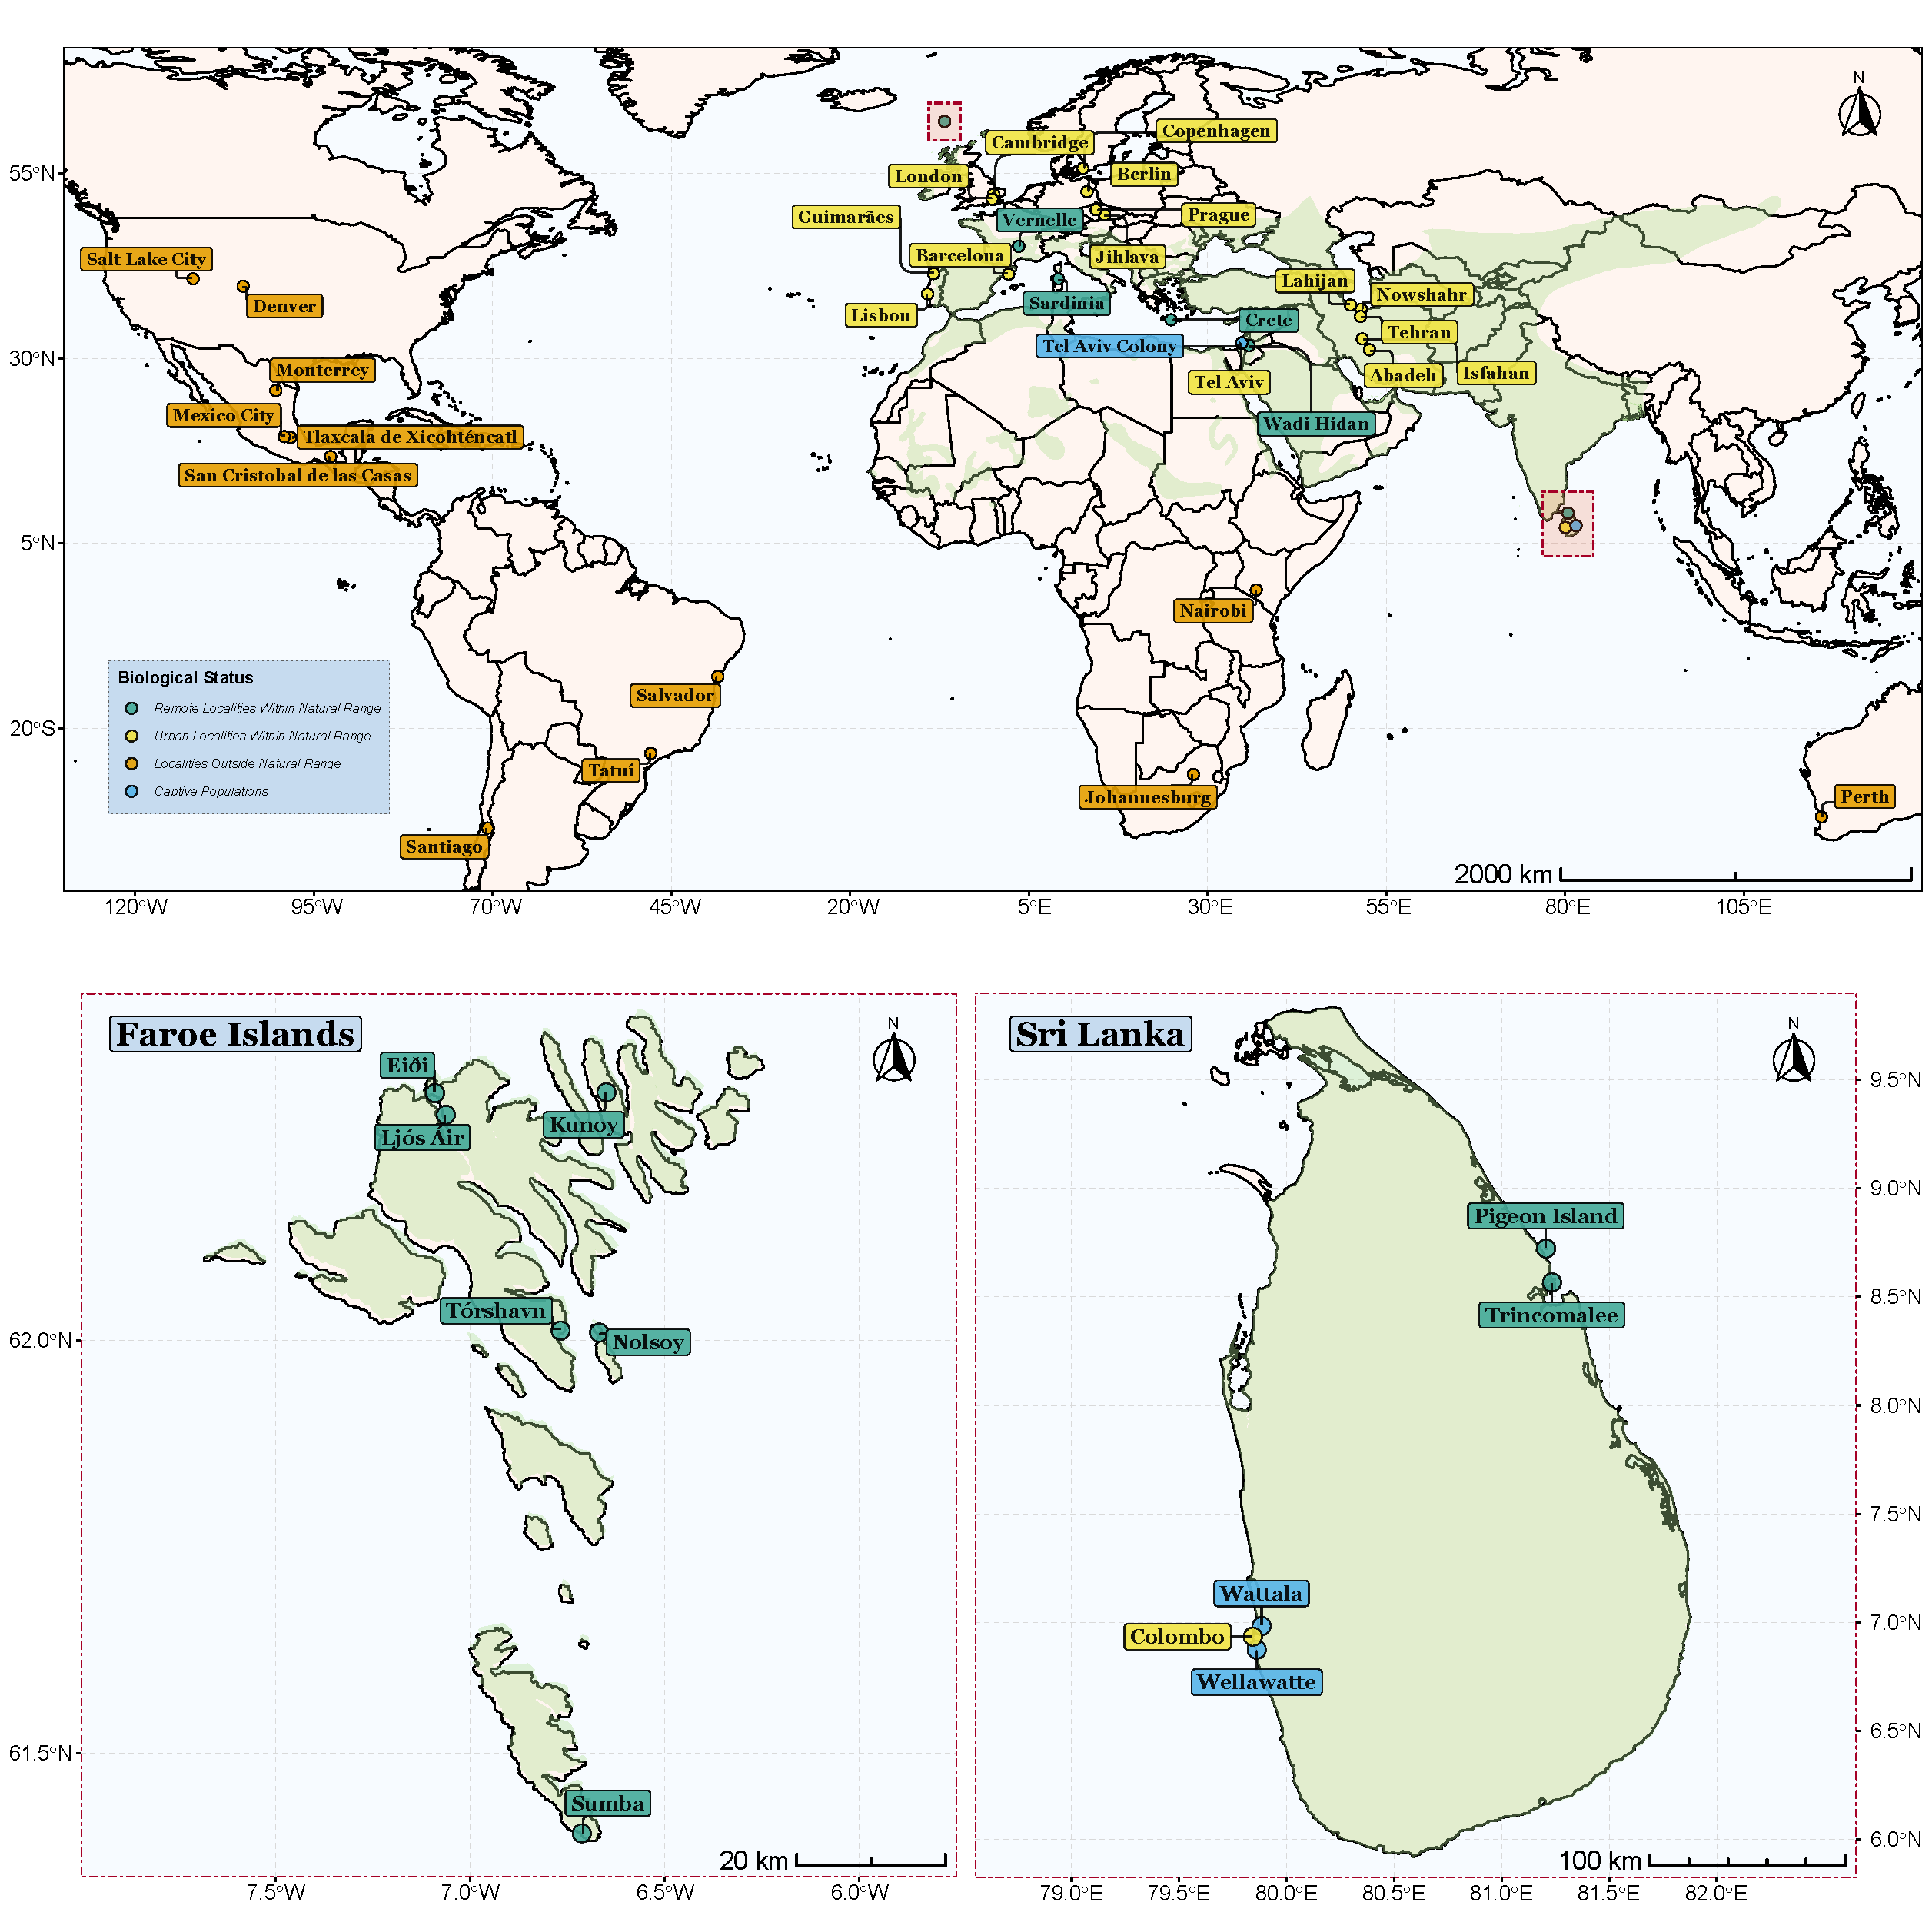
\includegraphics[scale=0.35]{../FPGP--Analyses/FPGP--Map/FPGP--Map.pdf}
\caption{Fitting of $r^2$ decay between called genotypes (CG) and genotype likelihoods (GL), across different simulated coverages (rows). The best-fitted curve (solid-line) and confidence interval (shaded area) was based on $250 bps$ bins but, for sake of clarity, data is represented as bins of $500 bps$ (points) and Y-axis us truncated at $0.5$. Confidence interval was based on 100 bootstraps.}
\label{MainText:FPGP--Map}
\end{figure}

\subsection{\textit{Sequencing Data and Filtering}}

\subsection{\textit{Population Genetics Statistics}}

\subsection{\textit{Phylogenetic Relationships Among Feral Pigeon Populations}}

\subsection{\textit{Population Structure Among Pigeon Populations}}

\subsection{\textit{Contribution of Pigeon Breeds to Current Non-domesticated Populations}}

% Discussion %

\section{Discussion}

% Methods %

\section{Methods}

\subsection{\textit{Sequencing Data Generation and Processing}}

\subsection{\textit{Data Analysis}}

\subsection{\textit{Population Genetics Statistics}}

\subsection{\textit{Phylogenetic Reconstruction}}

\subsection{\textit{Inference of Population Structure}}

\subsection{\textit{Contribution of Pigeon Breeds to Current Non-domesticated Populations}}


\bibliographystyle{natbib}
\bibliography{library}
\end{document}
